\section{Results and Discussion}
\label{sec:results}

The 26 datasets, ten seeds, four imbalance ratios, and five contamination
conditions (the shared clean condition plus four noise levels in each of the two
directions) form 9{,}360 stress cells. Nine methods (seven corrections plus the
two uncorrected baselines) are scored on every cell, giving 84{,}240 evaluations.
The three prior-dependent TabPFN corrections are also scored with the oracle
prior for diagnosis, adding 28{,}080 more. Of the 112{,}320 planned evaluations,
112{,}319 completed. The exception is \texttt{tabpfn\_downsample} on APS Failure
(seed 19, $r{=}0.10$, $c{=}0.05$, Direction A), which failed to converge
(Section~\ref{sec:methods-implementation}) and is excluded from the tables rather
than interpolated.

\subsection{Overall Correction Robustness}
\label{sec:results-rq1}

Every one of the seven correction methods produced at least one (dataset, $r$,
$c$, direction) block with negative Correction Gain, so no correction is
uniformly beneficial once label error is present. How often this happens varies
sharply by method. Table~\ref{tab:robustness} reports Correction Harm Rate (CHR)
and mean Correction Gain (CG, on balanced accuracy). \texttt{tabpfn\_threshold}
is the most robust method by both measures in both directions. Its CHR is 4.8\%
under Direction A and 2.4\% under Direction B, less than half the next-lowest
correction in either direction, and its mean CG (0.072 and 0.093) is the highest
of any method. The worst end of the table is the same in both directions.
\texttt{tabpfn\_distpfn} and \texttt{tabpfn\_distpfn\_t} have the highest CHR
under Direction A (35.1\% and 33.9\%) and, by a wider margin, under Direction B
(43.8\% and 47.4\%, more than five times the next-highest method there).

\begin{table}[t]
\centering
\caption{Correction Harm Rate and mean Correction Gain (balanced accuracy) over
noisy blocks ($c>0$), each averaged across ten seeds and pooled across datasets
and ratios ($n{=}416$ per method and direction).}
\label{tab:robustness}
\begin{tabular}{@{}lrrrr@{}}
\toprule
& \multicolumn{2}{c}{CHR} & \multicolumn{2}{c}{mean CG} \\
Method & Dir.\ A & Dir.\ B & Dir.\ A & Dir.\ B \\
\midrule
\texttt{xgb\_weighted}      & 0.130 & 0.060 & 0.026 & 0.034 \\
\texttt{xgb\_ros}           & 0.147 & 0.067 & 0.026 & 0.035 \\
\texttt{xgb\_smote}         & 0.135 & 0.072 & 0.023 & 0.033 \\
\texttt{tabpfn\_threshold}  & 0.048 & 0.024 & 0.072 & 0.093 \\
\texttt{tabpfn\_distpfn}    & 0.351 & 0.438 & 0.009 & $-$0.004 \\
\texttt{tabpfn\_distpfn\_t} & 0.339 & 0.474 & 0.008 & $-$0.009 \\
\texttt{tabpfn\_downsample} & 0.204 & 0.077 & 0.054 & 0.073 \\
\bottomrule
\end{tabular}
\end{table}

CHR counts any negative gain as a failure, including differences too small to
reflect more than measurement noise. Requiring a drop of at least 0.01
balanced-accuracy points lowers every rate sharply but does not change the
ranking. \texttt{tabpfn\_threshold} falls to 0.2\% (Dir.\ A) and 0.0\% (Dir.\ B),
every XGBoost method falls to 2.4\% or below, and \texttt{tabpfn\_downsample}
falls to 6.5\%/1.4\%. The DistPFN pair is the exception, at 13.9\%/13.2\% under
Direction A and 28.9\%/28.9\% under Direction B, four to over a hundred times any
other method's rate at that threshold.

Figure~\ref{fig:gain-heatmap} shows the same contrast across every tested $r$ and
$c$. \texttt{tabpfn\_threshold}'s gain stays positive across the grid in both
directions. \texttt{tabpfn\_distpfn}'s harm is uneven. Under Direction B it is
negative across nearly the whole $r{=}0.50$ row regardless of noise level, and
turns positive only at lower ratios. Under Direction A the picture is milder,
with the clearest positive gain at high $c$ and low $r$.

\begin{figure*}[t]
\centering
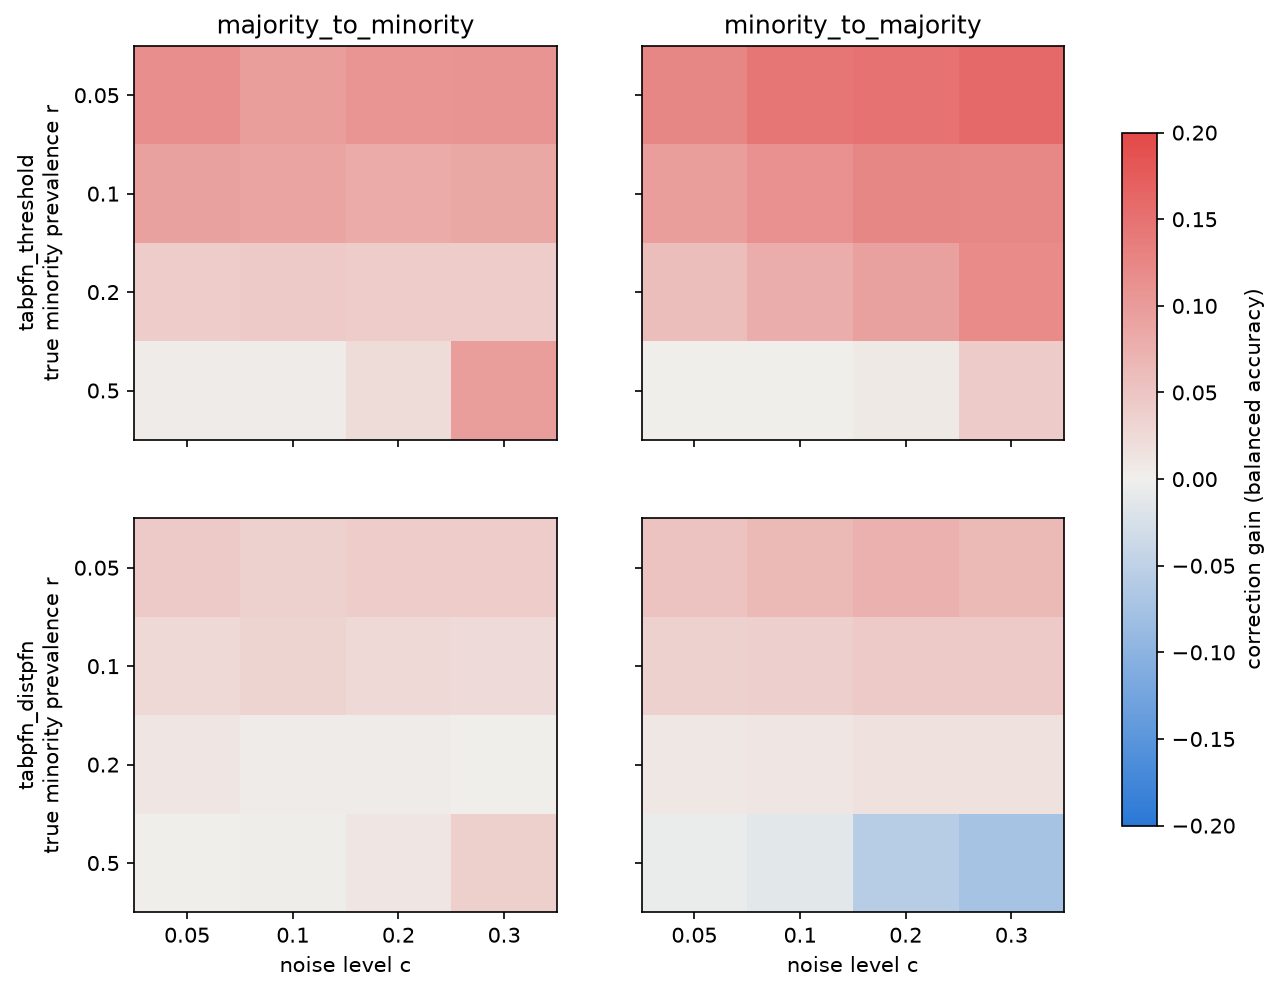
\includegraphics[width=0.85\linewidth]{figures/gain_heatmap_pair.png}
\caption{Correction gain (balanced accuracy) across $r$ and $c$ for
\texttt{tabpfn\_threshold} (top) and \texttt{tabpfn\_distpfn} (bottom), pooled
across 26 datasets and ten seeds. Blue marks cells where the correction hurt,
and red marks cells where it helped.}
\label{fig:gain-heatmap}
\end{figure*}

\subsection{Simplicity Outperforms Sophistication}
\label{sec:discussion-simplicity}

\texttt{tabpfn\_threshold} does less than any other correction. It shifts the
decision boundary from 0.5 to the class prior and nothing more
(Section~\ref{sec:methods-corrections}). It is nevertheless the most robust method
on discrimination (Table~\ref{tab:robustness}, Section~\ref{sec:results-rq1}),
with the lowest CHR and highest mean CG in both directions, and it leads on
break-even share too (Table~\ref{tab:breakeven}). Its calibration matches its
baseline by construction, since a threshold shift does not touch the predicted
probabilities (Section~\ref{sec:discussion-calibration} returns to why that is
not the same as leading on calibration). The two DistPFN variants sit at the
opposite end, with the highest CHR of any method in \emph{both} directions.

This builds on prior work. Elor and Averbuch-Elor~\cite{elor2022smote} found that
on clean data a well-tuned classifier often gains nothing from balancing and can
lose performance from it. This study shows that the same pattern holds, and
sharpens, once label noise is added. A correction can actively backfire, and in
this comparison the two most elaborate corrections backfire hardest on
discrimination while the simplest backfires least. Much of that backfiring is
concentrated at the balanced control $r{=}0.50$. Restricted to genuinely
imbalanced training sets ($r{\neq}0.50$), the DistPFN pair's Direction B CHR falls
from 43.8\%/47.4\% to 29.8\%/37.8\%, still four to twelve times
\texttt{tabpfn\_threshold}'s 0.3\% there (Section~\ref{sec:results-r050}). The
ranking does not change at any scope. A practitioner optimizing balanced accuracy
under uncertain label quality has, on these results, no clear reason to prefer a
more elaborate posterior-rescaling method over a threshold shift. That
recommendation does not cover every deployment, a point
Section~\ref{sec:discussion-calibration} returns to.

This may also reflect the study design. The severe-imbalance conditions combine
imbalance with a train/test prior mismatch, and threshold correction, DistPFN,
and DistPFN-T all target that mismatch. This may explain part of why
prior-adjusting corrections outperform resampling and cost-sensitive weighting in
general. It does not explain why the DistPFN variants fail more often than plain
threshold correction, which points to contamination robustness specifically.

\subsection{Robustness Check: Isolating the Balanced Control Condition ($r{=}0.50$)}
\label{sec:results-r050}

The headline numbers pool all four ratios, including $r{=}0.50$, a balanced
training set before contamination. To isolate it, every contribution metric and
statistical test is recomputed on $r \in \{0.20, 0.10, 0.05\}$ (hereafter
$r{\neq}0.50$) and on $r{=}0.50$ alone, using the same formulas and the same
already-collected evaluations. No model was retrained or re-scored.

Table~\ref{tab:robustness-r050} reports CHR and mean CG on $r{\neq}0.50$.
\texttt{tabpfn\_threshold} is unaffected in standing, and its Direction B CHR
falls from 2.4\% to 0.3\%. The DistPFN variants change substantially but not
completely. Under Direction B their pooled CHR of 43.8\%/47.4\% falls to 29.8\%
(\texttt{tabpfn\_distpfn}) and 37.8\% (\texttt{tabpfn\_distpfn\_t}) on
$r{\neq}0.50$, and their mean CG rises from $-0.004$/$-0.009$ pooled to
0.013/$-0.004$. At $r{=}0.50$ alone the same two methods fail 85.6\% and 76.0\% of
the time under Direction B, with mean gains of $-0.055$ and $-0.023$, and they
rarely reach break-even there (3.8\% of (dataset, $r{=}0.50$) pairs for both,
versus 46.2\%/47.4\% at $r{\neq}0.50$). Under Direction A the change is small. The
DistPFN pair's CHR moves from 35.1\%/33.9\% pooled to 34.9\%/35.9\%.
\texttt{tabpfn\_downsample}'s Direction A CHR does not fall when $r{=}0.50$ is
excluded (20.4\% pooled vs.\ 18.6\%), consistent with
Section~\ref{sec:discussion-direction}.

\begin{table}[t]
\centering
\caption{Correction Harm Rate and mean Correction Gain (balanced accuracy)
restricted to the imbalanced subset $r \in \{0.20, 0.10, 0.05\}$ ($n{=}312$ per
method and direction). Directly comparable to Table~\ref{tab:robustness}.}
\label{tab:robustness-r050}
\begin{tabular}{@{}lrrrr@{}}
\toprule
& \multicolumn{2}{c}{CHR} & \multicolumn{2}{c}{mean CG} \\
Method & Dir.\ A & Dir.\ B & Dir.\ A & Dir.\ B \\
\midrule
\texttt{xgb\_weighted}      & 0.115 & 0.032 & 0.028 & 0.043 \\
\texttt{xgb\_ros}           & 0.115 & 0.026 & 0.029 & 0.044 \\
\texttt{xgb\_smote}         & 0.106 & 0.029 & 0.026 & 0.041 \\
\texttt{tabpfn\_threshold}  & 0.032 & 0.003 & 0.084 & 0.119 \\
\texttt{tabpfn\_distpfn}    & 0.349 & 0.298 & 0.009 & 0.013 \\
\texttt{tabpfn\_distpfn\_t} & 0.359 & 0.378 & 0.004 & $-$0.004 \\
\texttt{tabpfn\_downsample} & 0.186 & 0.051 & 0.061 & 0.094 \\
\bottomrule
\end{tabular}
\end{table}

The Prior Sensitivity pattern changes too. At $r{=}0.50$, mean PSG for the DistPFN
pair under Direction A falls to $-0.058$/$-0.059$. On $r{\neq}0.50$ it turns
slightly positive ($+0.010$, $+0.009$), so the oracle prior modestly helps once
the balanced control is excluded. It remains negative under Direction B
($-0.013$, $-0.009$) and for \texttt{tabpfn\_threshold} in both directions
regardless of $r$. Every Friedman omnibus test remains significant on both the
$r{\neq}0.50$ and $r{=}0.50$-only subsets at both blocking levels ($p<10^{-8}$
throughout).

The core claims survive this check. No correction is uniformly safe, method
identity significantly affects balanced accuracy in every family and direction
with or without $r{=}0.50$, and \texttt{tabpfn\_threshold} remains the most robust
method, more clearly so once the balanced control is removed. What changes is the
size of the DistPFN pair's Direction B failure. A real share of it, though not
the majority, is a property of the balanced condition. Excluding $r{=}0.50$ cuts
the pair's Direction B CHR by roughly a third (43.8\%$\to$29.8\% and
47.4\%$\to$37.8\%), not down to the low single digits.

\subsection{Direction-Dependent Failure}
\label{sec:results-rq2}
\label{sec:discussion-direction}

Failure rates differ substantially between the two directed mechanisms, and the
direction of the difference depends on the method. Five of the seven methods have
a higher CHR under Direction A (majority rows relabeled as minority) than under
Direction B (minority rows relabeled as majority). These are \texttt{xgb\_ros},
\texttt{xgb\_smote}, \texttt{xgb\_weighted}, \texttt{tabpfn\_downsample}, and
\texttt{tabpfn\_threshold}, the last two by a wide margin
(Table~\ref{tab:robustness}). The two DistPFN variants show the opposite pattern.
Figure~\ref{fig:chr-regret} shows CHR and mean regret by method and direction.

This asymmetry is what class-conditional and asymmetric label-noise formalizations
predict~\cite{natarajan2013noisylabels,scott2013asymmetricnoise}, but it is large
enough to matter. A method's CHR under one direction is a poor predictor of its
CHR under the other. \texttt{tabpfn\_downsample}'s CHR is 20.4\% under Direction A
and 7.7\% under Direction B, nearly a threefold difference for the same method on
the same datasets. A robustness claim validated under one corruption mechanism, or
under symmetric random flips, does not transfer to a directed, class-conditional
error, and the true direction of label error is rarely known in advance. This is
the strongest argument in the study for testing every correction under both
directions.

\begin{figure*}[t]
\centering
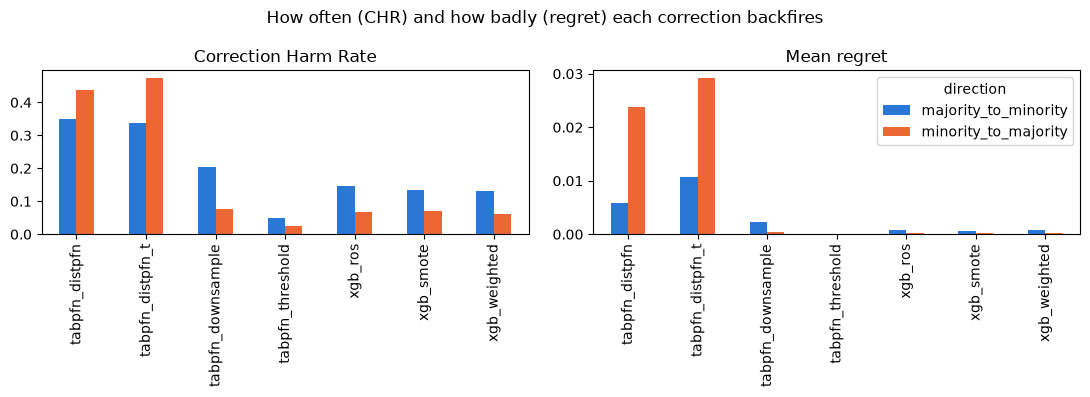
\includegraphics[width=0.85\linewidth]{figures/chr_regret.png}
\caption{Correction Harm Rate (left) and mean regret (right, $\max(0,-\text{CG})$)
by method and direction, over noisy blocks pooled across 26 datasets.}
\label{fig:chr-regret}
\end{figure*}

Regret and CHR tell a consistent story. The DistPFN pair has both the highest CHR
and the highest mean regret in both directions. Under Direction A,
\texttt{tabpfn\_distpfn\_t}'s mean regret (0.0108) is the highest of any method,
ahead of \texttt{tabpfn\_distpfn} (0.0059) and \texttt{tabpfn\_downsample}
(0.0023), even though \texttt{tabpfn\_downsample}'s CHR (20.4\%) sits below the
DistPFN pair's 33.9--35.1\%. Under Direction B the regret of
\texttt{tabpfn\_distpfn\_t} (0.0292) and \texttt{tabpfn\_distpfn} (0.0239) is an
order of magnitude above every other method, all of which are at 0.0004 or below.
\texttt{tabpfn\_threshold} has the lowest regret in both directions (0.0001 and
0.0000).

Part of this asymmetry traces to the uncorrected baselines. From $c{=}0$ to
$c{=}0.30$, balanced accuracy of \texttt{xgb\_none} falls by 0.076 (0.741 to 0.665)
under Direction B, against 0.034 (0.741 to 0.707) under Direction A, roughly 2.2
times as much. \texttt{tabpfn\_none} shows the same pattern, 0.066 against 0.032,
roughly 2.0 times. Losing genuine minority rows is more damaging to an uncorrected
model than diluting the minority class with mislabeled majority rows. This helps
explain why a correction's robustness under one direction does not predict its
robustness under the other.

\subsection{Break-Even Contamination Rates}
\label{sec:results-rq3}

Table~\ref{tab:breakeven} gives, for each method and direction, the share of the
104 (dataset, $r$) combinations (26 datasets $\times$ 4 ratios) whose
seed-averaged gain never drops to zero or below within the tested range, that is,
$c^*>0.30$. \texttt{tabpfn\_threshold} leads here too, staying net-beneficial
through the full range in 85.6\% of Direction A conditions and 87.5\% of Direction
B conditions. The lowest shares in both directions belong to the DistPFN pair,
40.4\% for \texttt{tabpfn\_distpfn} under Direction A and 32.7\% for
\texttt{tabpfn\_distpfn\_t} under Direction B. CHR counts every failing block
individually. Break-even share asks only whether a method's seed-averaged trend,
within one (dataset, $r$) combination, ever crosses zero. The two measures mostly,
but not perfectly, agree, which is why Section~\ref{sec:methods-contribution}
keeps CHR, Regret, and $c^*$ separate.

\begin{table}[t]
\centering
\caption{Share of (dataset, $r$) conditions, out of 104, where a method's
seed-averaged Correction Gain never dropped to zero or below within the tested
contamination range ($c^*>0.30$).}
\label{tab:breakeven}
\begin{tabular}{@{}lrr@{}}
\toprule
Method & Dir.\ A & Dir.\ B \\
\midrule
\texttt{xgb\_weighted}      & 69.2\% & 80.8\% \\
\texttt{xgb\_ros}           & 64.4\% & 80.8\% \\
\texttt{xgb\_smote}         & 62.5\% & 78.8\% \\
\texttt{tabpfn\_threshold}  & 85.6\% & 87.5\% \\
\texttt{tabpfn\_distpfn}    & 40.4\% & 37.5\% \\
\texttt{tabpfn\_distpfn\_t} & 41.3\% & 32.7\% \\
\texttt{tabpfn\_downsample} & 62.5\% & 74.0\% \\
\bottomrule
\end{tabular}
\end{table}

The corrupted prior explains less of a correction's failure than expected. On
average, the deployable observed-prior variant slightly outperforms the oracle
diagnostic rather than trailing it. Table~\ref{tab:psg} gives mean PSG
(Equation~\ref{eq:psg}) pooled and at $c{=}0.30$. Pooled, it is negative for all
three prior-dependent methods in both directions. The gap is not fixed, however.
At $c{=}0.30$ alone, \texttt{tabpfn\_threshold}'s mean PSG under Direction A is the
widest of the three, even though it is the most robust method on balanced
accuracy, so the ranking of prior sensitivity across methods is not stable.

\begin{table}[t]
\centering
\caption{Mean Prior Sensitivity Gap (Equation~\ref{eq:psg}), pooled across noisy
blocks and at $c{=}0.30$. Negative throughout: the oracle prior does not reliably
outperform the observed one.}
\label{tab:psg}
\begin{tabular}{@{}lrr@{}}
\toprule
Method / Direction & mean PSG (pooled) & mean PSG ($c{=}0.30$) \\
\midrule
\texttt{tabpfn\_threshold}, Dir.\ A  & $-0.012$ & $-0.037$ \\
\texttt{tabpfn\_threshold}, Dir.\ B  & $-0.008$ & $-0.019$ \\
\texttt{tabpfn\_distpfn}, Dir.\ A    & $-0.007$ & $-0.033$ \\
\texttt{tabpfn\_distpfn}, Dir.\ B    & $-0.020$ & $-0.043$ \\
\texttt{tabpfn\_distpfn\_t}, Dir.\ A & $-0.008$ & $-0.036$ \\
\texttt{tabpfn\_distpfn\_t}, Dir.\ B & $-0.014$ & $-0.033$ \\
\bottomrule
\end{tabular}
\end{table}

Figure~\ref{fig:psg} shows the observed and oracle curves. At low contamination they
stay close together. The two DistPFN variants separate sharply above $c{=}0.20$
under Direction A, with the oracle degrading faster, while
\texttt{tabpfn\_threshold} shows a comparable or larger separation at the highest
noise level. Even the true prior does not fully recover clean-condition performance
under severe contamination.

\begin{figure*}[t]
\centering
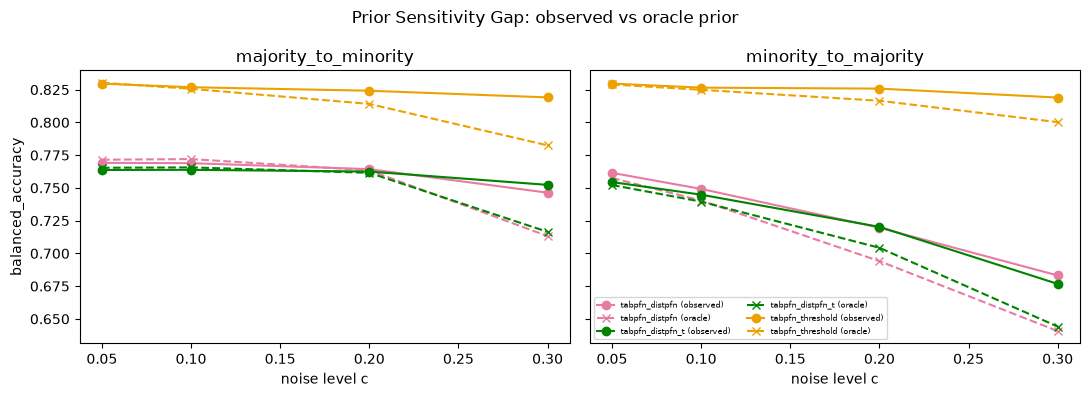
\includegraphics[width=0.85\linewidth]{figures/oracle_vs_observed.png}
\caption{Observed-prior (deployable, solid) versus oracle-prior (diagnostic,
dashed) balanced accuracy for the three prior-dependent TabPFN methods, pooled
across 26 datasets.}
\label{fig:psg}
\end{figure*}

\subsection{The Corrupted Prior Is Not the Main Failure Mode}
\label{sec:discussion-prior}

\label{sec:results-rq4}
The most surprising result is that mean PSG is negative for all three
prior-dependent methods in both directions. The true prior, which no deployment
could supply, does not reliably outperform the corrupted one. If the wrong prior
were the primary cause of these methods' decline, correcting it should have helped.
It does not, at least not under Direction B, or under Direction A at high
contamination. Restricted to $r{\neq}0.50$, mean PSG turns positive for both DistPFN
variants under Direction A ($+0.010$, $+0.009$). The corrupted prior therefore
contributes to their Direction A decline once the balanced control is excluded. It
is not the dominant effect that the more strongly negative figure at $r{=}0.50$
alone ($-0.058$/$-0.059$) suggests (Section~\ref{sec:results-r050}). The claim that
the corrupted prior is not the primary failure mode is strongest under Direction B,
increasingly so at high contamination for \texttt{tabpfn\_threshold}, and more
qualified for the DistPFN pair under Direction A at moderate contamination.

A structural reason follows from how these corrections work. All three adjust
TabPFN's output probabilities after the fact, using the class
prior~\cite{saerens2002adjusting,lee2026distpfn}. None of them touches the training
rows TabPFN reads as its in-context prompt~\cite{hollmann2023tabpfn,hollmann2025tabpfnv2}.
Contamination happens before any correction is applied, so the mislabeled rows stay
in that prompt whichever prior is supplied afterward. Swapping in the true prior
fixes the summary statistic the correction uses, but not the individual wrong
examples TabPFN has already been shown. This would explain why the oracle prior
helps so little. Confirming it would require an experiment this study did not run,
comparing a prior-only fix against a fix that also removes the mislabeled rows from
the context.

\subsection{Statistical Significance}
\label{sec:results-significance}

Table~\ref{tab:friedman} reports the Friedman omnibus test for each family and
direction, blocked by (dataset, $r$, $c$) ($n{=}416$). All four are significant at
$p<10^{-85}$, so method identity significantly affects balanced accuracy within both
families in both directions.

\begin{table}[t]
\centering
\caption{Friedman omnibus test statistics by family and direction. Condition
blocks are (dataset, $r$, $c$), $n{=}416$. Dataset blocks are one per dataset,
$n{=}26$, the more conservative check.}
\label{tab:friedman}
\label{tab:friedman-dataset}
\begin{tabular}{@{}llrrrr@{}}
\toprule
& & \multicolumn{2}{c}{Condition blocks} & \multicolumn{2}{c}{Dataset blocks} \\
Family & Direction & $\chi^2$ & $p$ & $\chi^2$ & $p$ \\
\midrule
XGBoost & Dir.\ A & 400.0 & $2.2\times10^{-86}$ & 46.8 & $3.7\times10^{-10}$ \\
XGBoost & Dir.\ B & 563.7 & $7.3\times10^{-122}$ & 47.4 & $2.9\times10^{-10}$ \\
TabPFN  & Dir.\ A & 681.7 & $3.1\times10^{-146}$ & 69.4 & $3.0\times10^{-14}$ \\
TabPFN  & Dir.\ B & 933.0 & $1.2\times10^{-200}$ & 71.5 & $1.1\times10^{-14}$ \\
\bottomrule
\end{tabular}
\end{table}

Blocking by (dataset, $r$, $c$) treats conditions from the same dataset as
independent evidence, although they share that dataset's feature distribution and
test set. The right-hand columns of Table~\ref{tab:friedman} repeat the comparison
with each dataset as a single block ($n{=}26$), the more conservative standard for comparing algorithms
across datasets (Section~\ref{sec:methods-statistics}). The $p$-values rise from
below $10^{-85}$ to between $10^{-14}$ and $10^{-9}$, but all four stay far below the
conventional $p<0.05$. Method identity affects balanced accuracy either way. The
(dataset, $r$, $c$) version overstates how strong that evidence is, not whether it
exists.

Pairwise tests (Holm-corrected) show where the differences lie. At the (dataset, $r$,
$c$) level, every uncorrected baseline differs significantly from every correction in
its family under Direction A. Under Direction B this holds for every XGBoost
correction and for \texttt{tabpfn\_threshold} and \texttt{tabpfn\_downsample}. Neither
DistPFN variant differs significantly from \texttt{tabpfn\_none} under Direction B
($p_{\text{Holm}}=0.58$ and $0.87$), despite their pooled CHR of 43.8\%/47.4\%. At the
dataset level, \texttt{tabpfn\_threshold} still differs significantly from every other
TabPFN method in both directions, so the finding that it is the most robust method
survives. The three XGBoost corrections become mutually indistinguishable in both
directions, though each still differs from \texttt{xgb\_none}. Under Direction B,
\texttt{tabpfn\_none}, \texttt{tabpfn\_distpfn}, and \texttt{tabpfn\_distpfn\_t} are
mutually indistinguishable ($p_{\text{Holm}}=1.00$ for all pairs). Under Direction A,
\texttt{tabpfn\_distpfn} is not significantly different from \texttt{tabpfn\_none}
($p_{\text{Holm}}=0.07$), and the two DistPFN variants are no longer distinguishable
from each other ($p_{\text{Holm}}=0.12$). None of the descriptive measures, CHR, mean
CG, or break-even share, depends on these tests. What changes is which differences a
formal test can support at $n{=}26$. The DistPFN pair's Direction B failure is real
and large by descriptive measures, but not statistically distinguishable from the
null at the dataset-level standard.

\subsection{Calibration Reliability and Accuracy}
\label{sec:results-reliability}
\label{sec:discussion-calibration}

Figure~\ref{fig:reliability} tracks Brier score and expected calibration error (ECE)
against noise level. Every XGBoost correction improves on \texttt{xgb\_none} at every
noise level tested, in both directions. \texttt{tabpfn\_downsample} is worse-calibrated
than the uncorrected \texttt{tabpfn\_none} on both ECE and Brier score at every noise
level under Direction A, the only method in the study with that pattern on either
metric. \texttt{tabpfn\_threshold} never exceeds its baseline's Brier score or ECE in
either direction. This follows from how it works. It moves only the decision threshold,
so the probabilities that Brier score and ECE measure are identical to those of
\texttt{tabpfn\_none} by construction. \texttt{tabpfn\_distpfn} and
\texttt{tabpfn\_distpfn\_t} are the two best-calibrated methods of any tested, correction
or baseline, at every noise level in both directions. They also have the highest CHR on
balanced accuracy (Section~\ref{sec:results-rq1}). Discrimination and calibration are
therefore different failure modes. A correction that often underperforms its baseline on
discrimination can still assign well-calibrated probabilities.

\begin{figure*}[t]
\centering
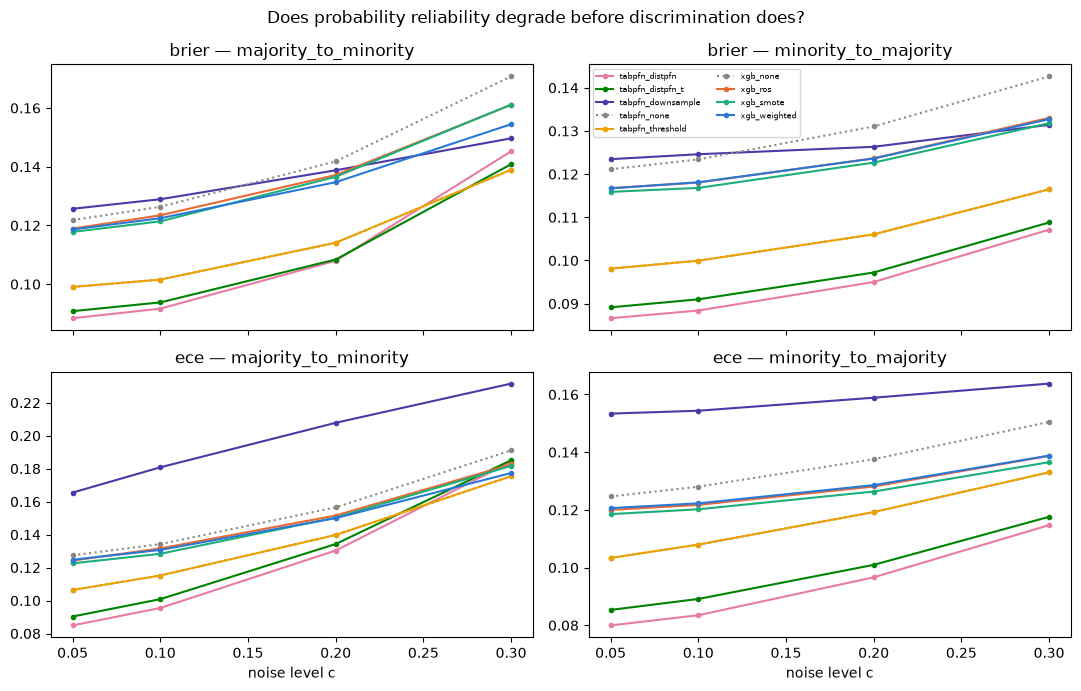
\includegraphics[width=0.85\linewidth]{figures/reliability.png}
\caption{Brier score (top) and expected calibration error (bottom) against noise level,
faceted by direction, pooled across 26 datasets. Dotted gray lines mark the two
uncorrected baselines.}
\label{fig:reliability}
\end{figure*}

Balanced accuracy and calibration measure different properties, and a correction can
excel at one while failing at the other. That matters for deployment. A system that
only needs a correct label cares mainly about discrimination, and by that standard the
DistPFN variants are a poor choice under contamination. A system that acts on predicted
probabilities, for example by setting a risk threshold, allocating a limited budget, or
ranking cases by urgency, cares about calibration first. For that use, the pair's CHR is
the wrong reason to rule them out. Reporting CHR and mean CG alone would also miss that
\texttt{tabpfn\_downsample} is uniquely poor on calibration under Direction A, even though
its balanced accuracy profile looks far more favorable there, with the second-highest
mean CG of any method. Deployment requires checking both axes separately rather than
inferring one from the other.

\subsection{Implications for Imbalance Correction Under Label Noise}
\label{sec:discussion-implications}

Related work on imbalance and label noise as a joint problem has proposed new
training-time algorithms: combining cleaning with resampling~\cite{koziarski2020ccr},
active learning with noisy-label training~\cite{khanal2024activelabel}, class-balanced
sample selection~\cite{liu2024imbalancednoisy}, or deliberately engineered label noise
that corrects a known class bias~\cite{hu2025beneficialnoise}. This study asks a
different question: whether the corrections practitioners already use need replacing at
all. The answer depends on which correction is in use. \texttt{tabpfn\_threshold} stays
net-beneficial through the full contamination range in 85.6\% to 87.5\% of conditions
(Table~\ref{tab:breakeven}), the highest share in both directions, so switching to it may
fix most of what a new algorithm would need to solve. The DistPFN variants fail badly on
discrimination under high contamination in both directions on the full pool, so for a
deployment that needs a correct label the case for joint noise-and-imbalance-aware
training remains strong. How this choice depends on the deployment's needs is set out in
Section~\ref{sec:discussion-calibration}. Telling these situations apart requires an
audit of this kind, not a default assumption that a published correction is safe or
unsafe on every axis a deployment cares about.